\section{Production Process Description} \label{sec:ProdProc}

Here the process to produce the parts are shown along with the assembly procedures, though all the parts of the seat are bought from the suppliers and our factory will only focus on the assembly. The overall production sequence is shown in Figure \ref{fig:ProdSeq}.

\begin{figure}[!htp]
    \centering
    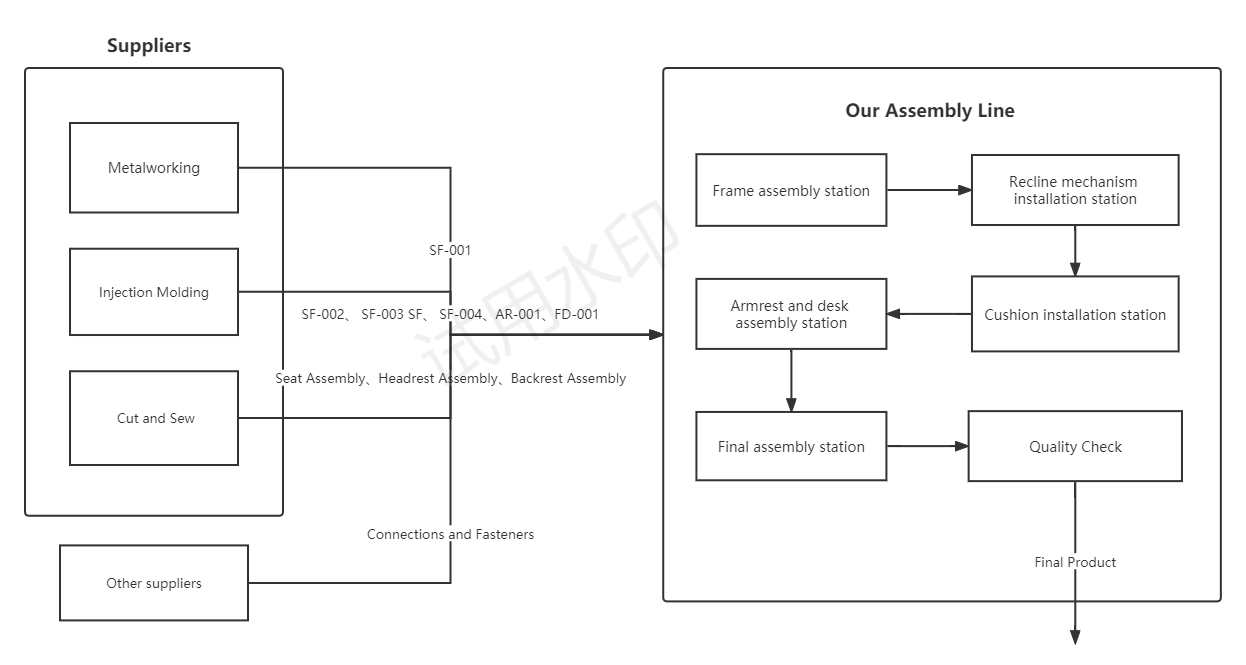
\includegraphics[width=\textwidth]{images/production sequence.png}
    \caption{Production Sequence}
    \label{fig:ProdSeq}
\end{figure}

\subsection{Metalworking}
In this procedure, the high-strength aluminum will be cut and shaped into the sticks we need (SF-001). The machines needed in this procedure are the saw and lathe, shown in Figure \ref{fig: saw} and Figure \ref{fig: lathe} respectively. The saw is used to cut the aluminum into the length we need, and the lathe is used to shape the aluminum into the shape we need. 

\begin{figure}[!htp]
    \centering
    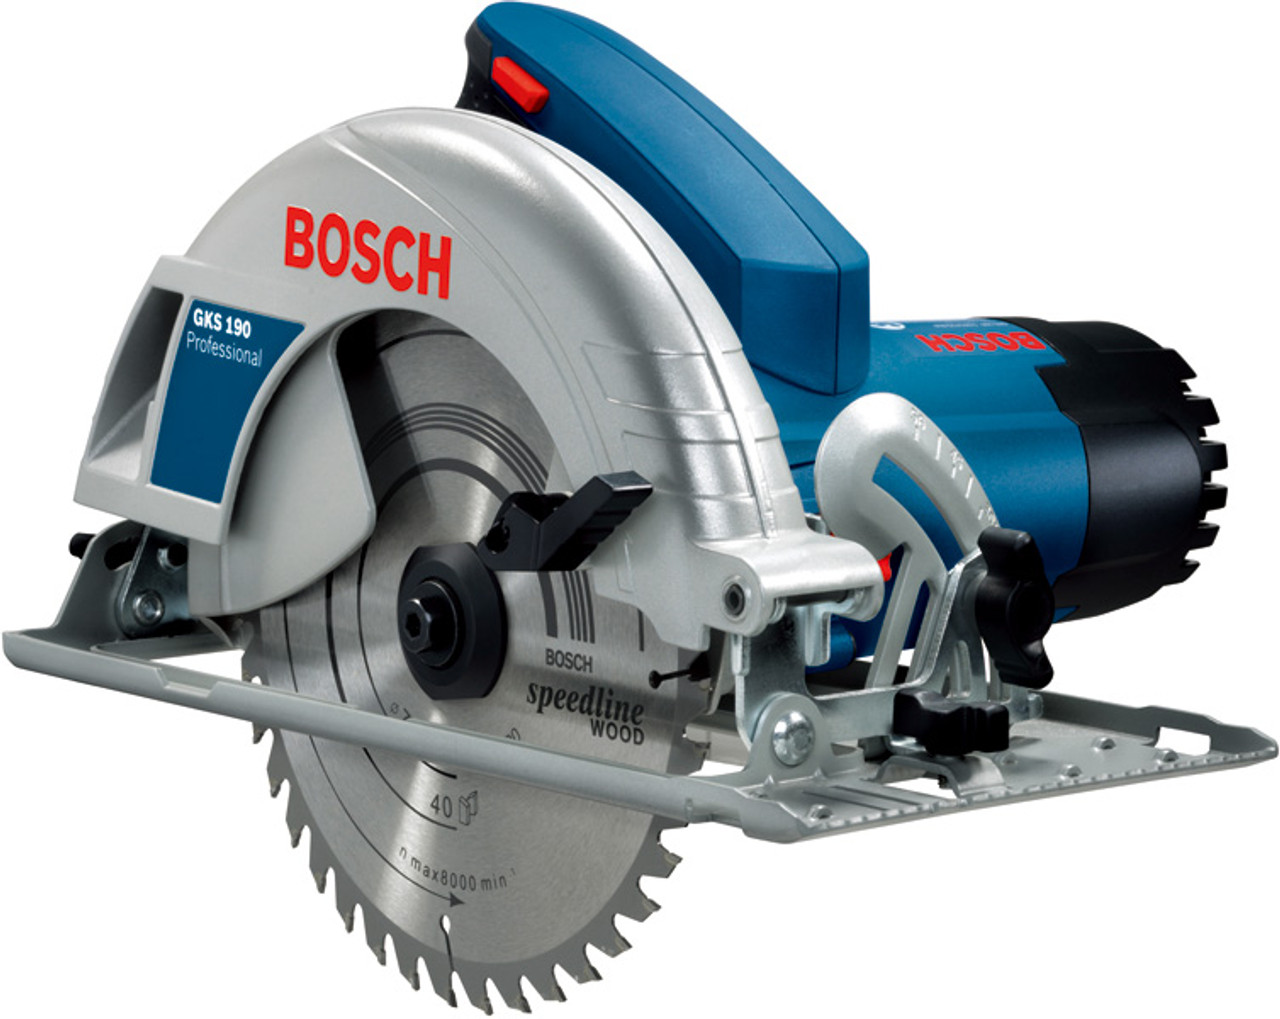
\includegraphics[width=0.6\textwidth]{images/saw.jpg}
    \caption{Saw machine}
    \label{fig: saw}
\end{figure}

\begin{figure}[!htp]
    \centering
    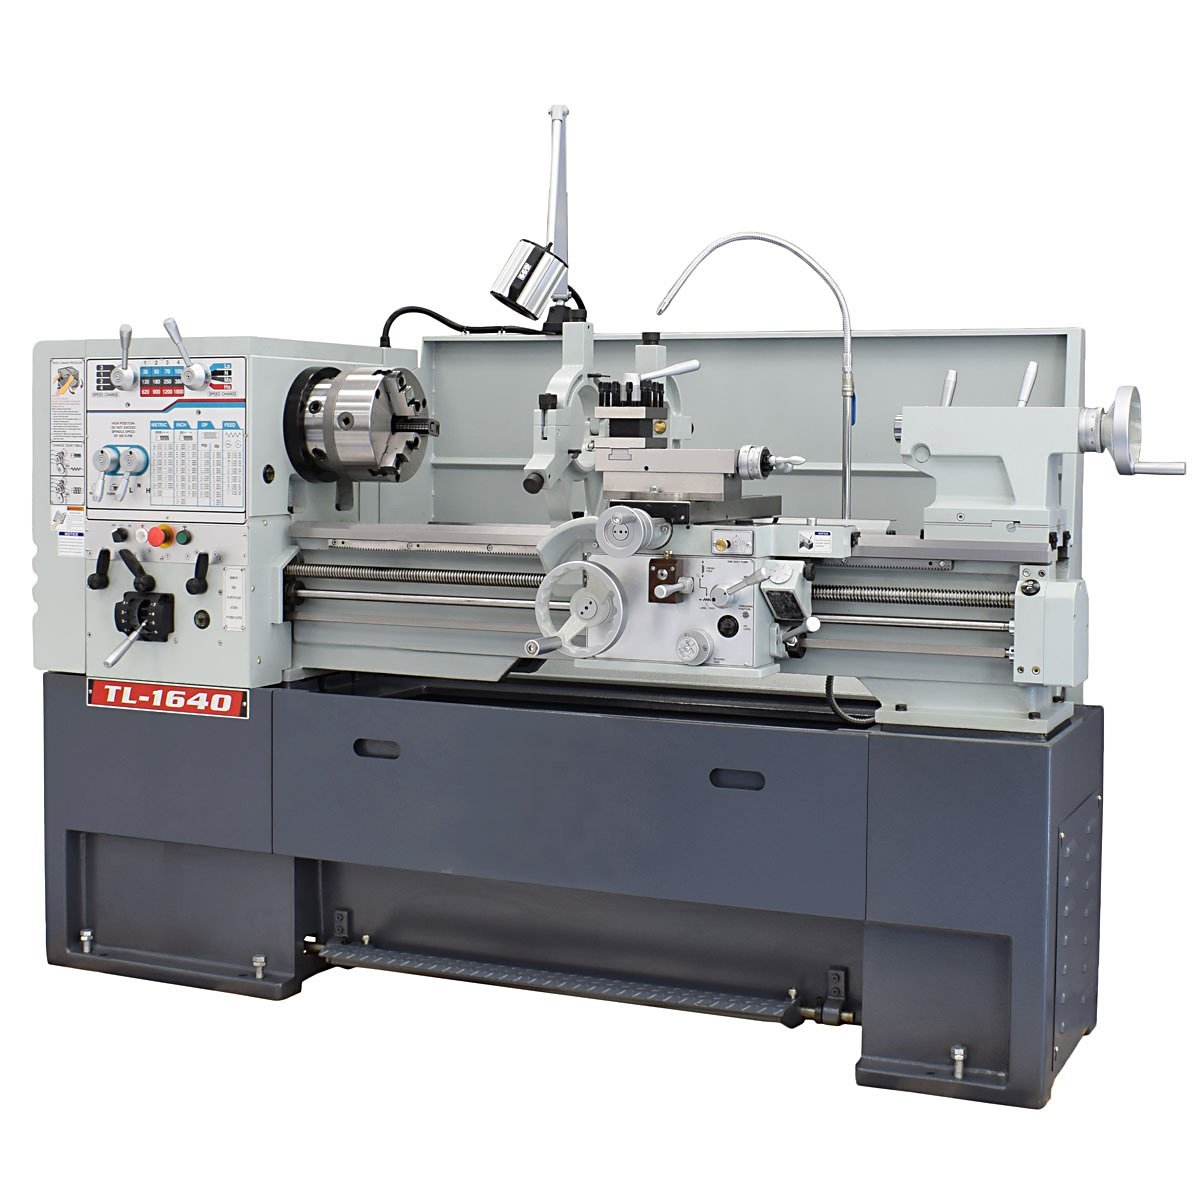
\includegraphics[width=0.6\textwidth]{images/lathe.jpg}
    \caption{Lathe machine}
    \label{fig: lathe}
\end{figure}

\subsection{Injection Molding}
In this procedure, the thermoplastics reinforced with carbon fibers (TRCF) will be processed and shaped into the parts we need (SF-002, SF-003, SF-004, AR-001 and FD-001). First, the TRCF material will be cut into small pellets or granules of uniform size that can be easily melted and molded. The TRCF material should also be properly dried to prevent moisture absorption and ensure consistent quality. Second, load the TRCF material into the hopper of an injection molding machine. The hopper will feed the material into a heated barrel for melting. Third, the TRCF material is heated and melted in the barrel of the injection molding machine. The temperature and pressure settings may vary depending on the specific TRCF material being used. Once the TRCF material is molten, it is injected into a mold cavity under high pressure. The mold is designed to produce the desired shape and size of the final product. Then, the TRCF material inside the mold is allowed to cool and solidify, taking the shape of the mold cavity. The cooling time and temperature depend on the thickness and complexity of the part being molded. After the TRCF material has solidified, the mold opens and the finished part is ejected from the mold cavity. Finally, the finished part may require trimming and finishing to remove any excess material or improve its surface quality. This can be done using various techniques such as cutting, sanding, or polishing.

During these steps, the industrial machines and tools include 
\begin{enumerate}
    \item Raw Material Preparation: Pelletizer, dryer
    \item Loading the Material: Injection molding machine with hopper and screw feeder
    \item Heating and Melting: Injection molding machine with heating elements, barrel, and screw
    \item Injection: Injection molding machine with mold clamping unit, injection unit, and nozzle
    \item Cooling and Solidification: Injection molding machine with cooling system, mold release agent, and mold temperature controller
    \item Ejection: Injection molding machine with ejector pins, knockout bars, and robotic arm (optionally)
    \item Trimming and Finishing: Cutting tool (such as a saw or cutter), sandpaper or polishing cloth or files.
\end{enumerate}
The machines needed are shown in Figure \ref{fig: pelletizer}, \ref{fig: injection}, \ref{fig: injection2}, \ref{fig: saw} and \ref{fig:cuodao}.

\begin{figure}[!htp]
    \centering
    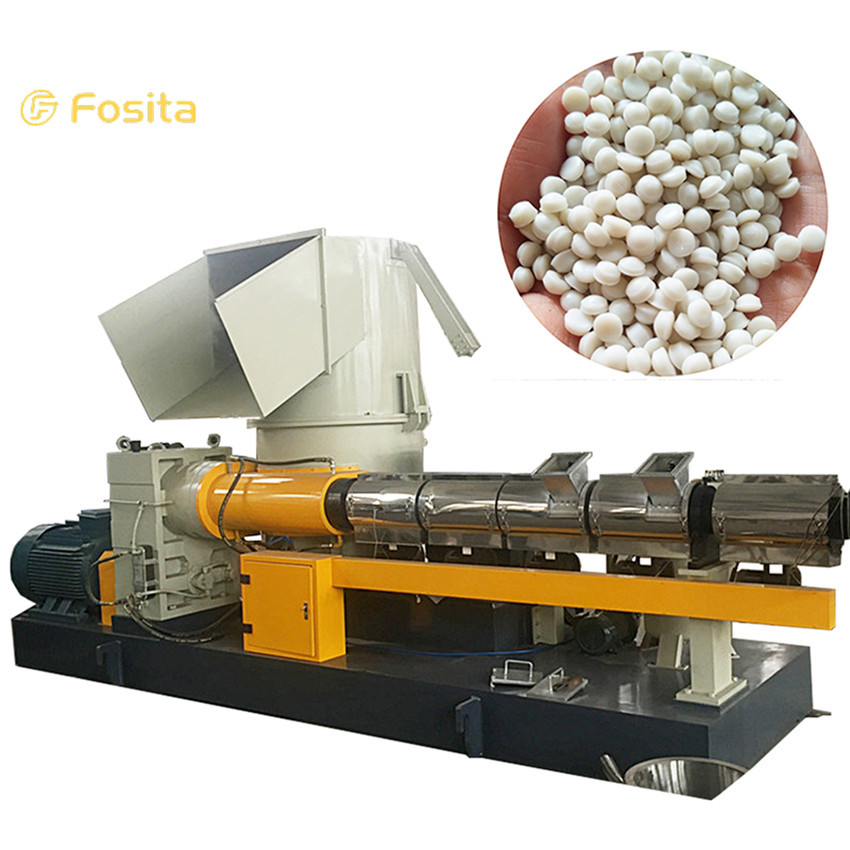
\includegraphics[width=0.6\textwidth]{images/Pelletizer.jpg}
    \caption{Pelletizer with dryer}
    \label{fig: pelletizer}
\end{figure}

\begin{figure}[!htp]
    \centering
    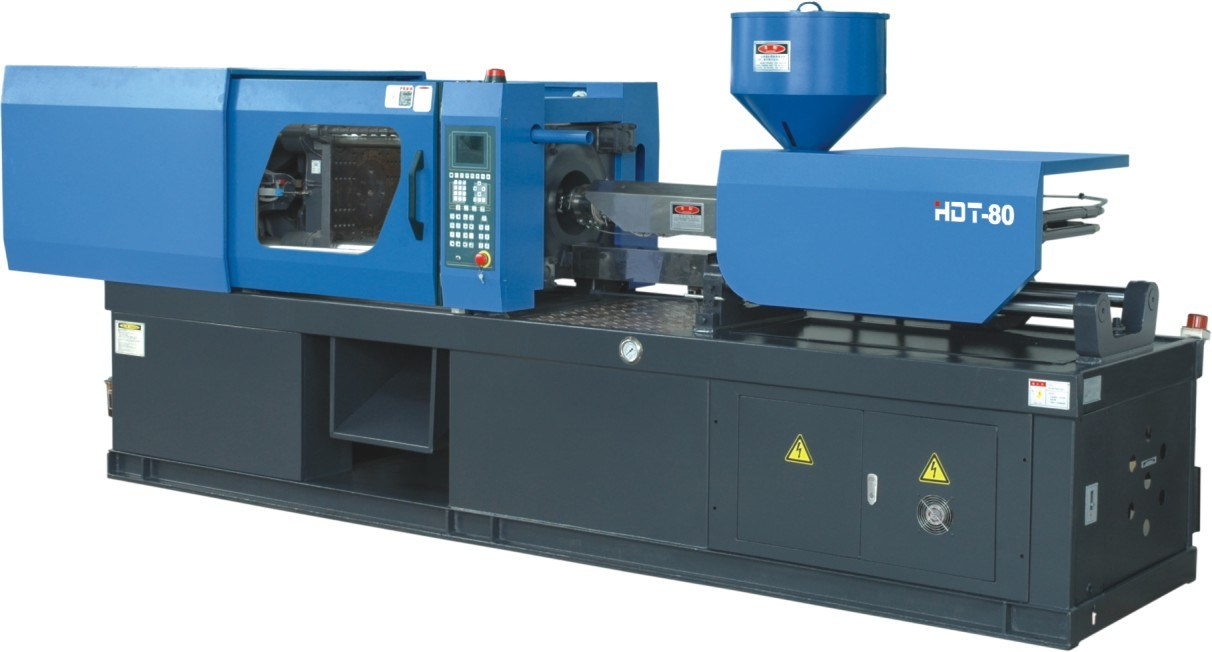
\includegraphics[width=0.6\textwidth]{images/Injection.jpg}
    \caption{Injection molding machine 1}
    \label{fig: injection}
\end{figure}

\begin{figure}[!htp]
    \centering
    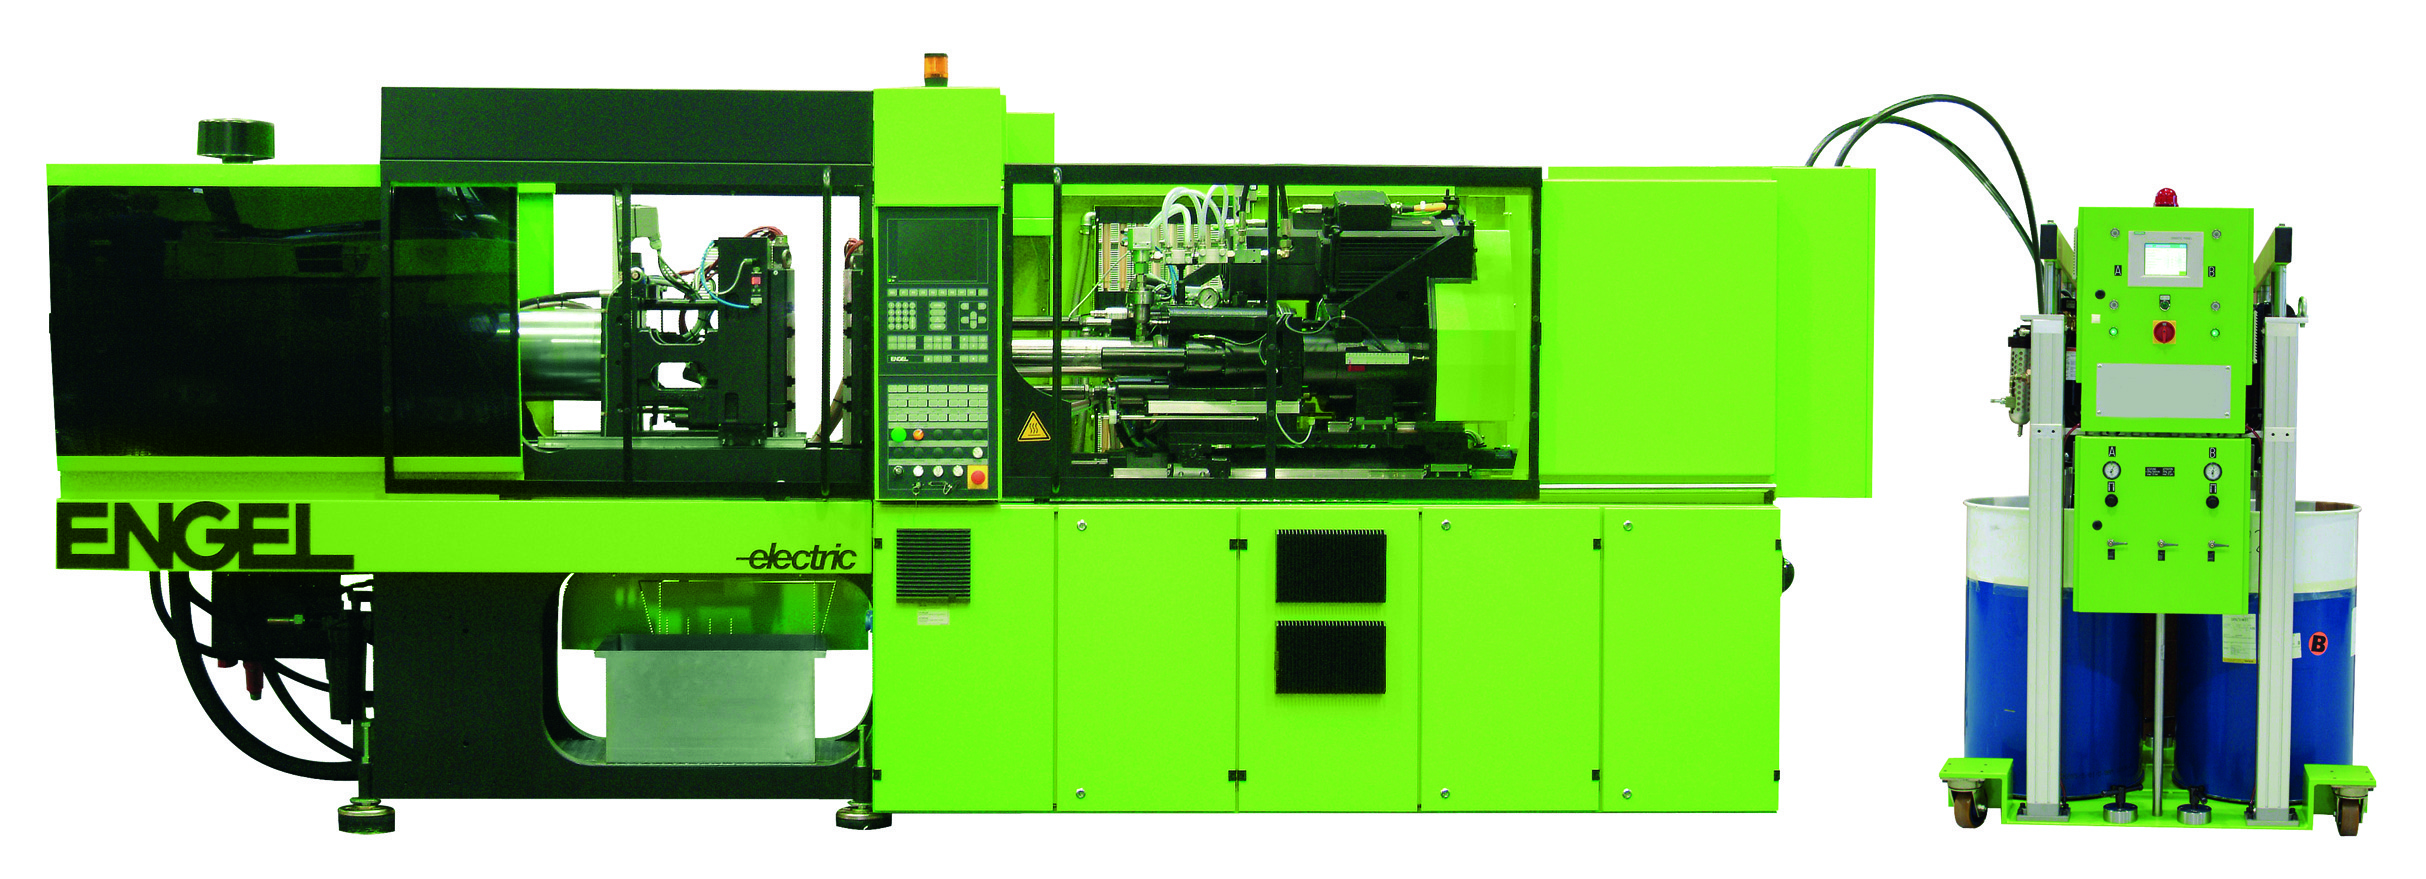
\includegraphics[width=0.6\textwidth]{images/Injection2.jpg}
    \caption{Injection molding machine 2}
    \label{fig: injection2}
\end{figure}

\begin{figure}
    \centering
    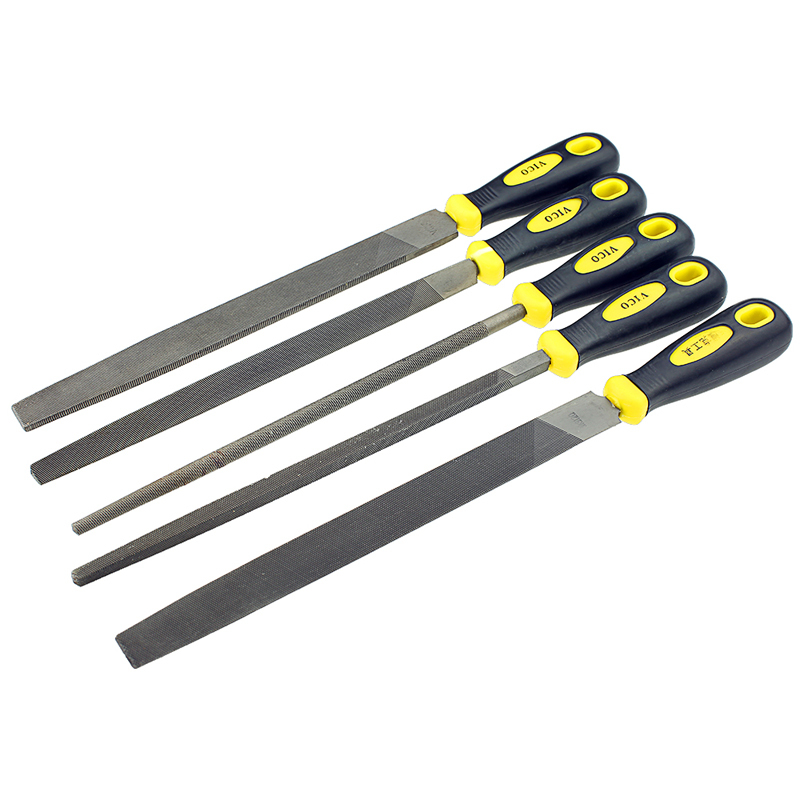
\includegraphics[width=0.6\textwidth]{images/cuodao.jpg}
    \caption{Finishing and polishing tool}
    \label{fig:cuodao}
\end{figure}

\subsection{Cut and Sew}
In this procedure, polyurethane foam and PU leather are shaped to make the seat assembly, backrest assembly and headrest assembly. First, measure and cut the polyurethane foam to fit the size and shape of the seat cushion needed. Then, place the cut polyurethane foam into a mold or shape it manually by carving, sanding, or cutting using appropriate tools. Once the polyurethane foam has been molded, cover it with a layer of batting or fabric to provide a smooth surface for the PU leather cover.

As for the PU leather, first, measure and cut the PU leather to fit the size and shape of the seat cover needed. Second, sew together the pieces of PU leather to form the cover of the seat cushion. Then, place the PU leather cover over the top of the polyurethane foam cushion and stretch it tightly around the foam to ensure a snug fit. Use an adhesive or staples to secure the edges of the PU leather cover to the underside of the foam cushion. Finally, finish the seat cushion by adding any necessary trimmings, such as piping or buttons.

The tools and machines typically used in these steps include (partly shown in Figures \ref{fig:carving}, \ref{fig:wire_cutter}, \ref{fig:sew} and \ref{fig:staple}),
\begin{enumerate}
    \item Measuring and Cutting: Measuring tape, sharp blade or utility knife
    \item Mold Polyurethane Foam: Grinding machine, sanding machine, carving tool, hot wire cutter
    \item Cover Polyurethane Foam: Staple gun, scissors
    \item Sew PU Leather: Sewing machine, thread
    \item Attach PU Leather Cover: Adhesive, staple gun
    \item Add Finishing Touches: Piping cord, button covering kit, decorative trim, etc.
\end{enumerate}

\begin{figure}[!htp]
    \centering
    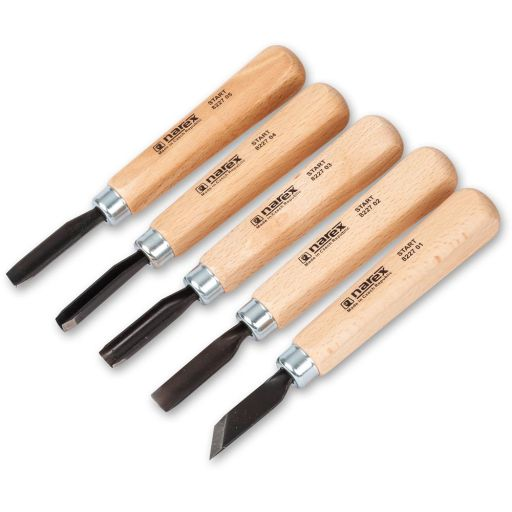
\includegraphics[width=0.6\textwidth]{images/carving tool.jpg}
    \caption{Carving tool}
    \label{fig:carving}
\end{figure}

\begin{figure}[!htp]
    \centering
    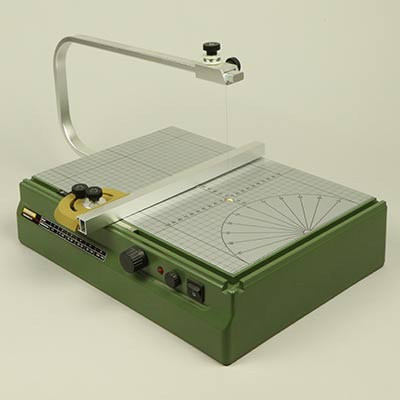
\includegraphics[width=0.6\textwidth]{images/hot wire cutter.jpg}
    \caption{Hot wire cutter}
    \label{fig:wire_cutter}
\end{figure}


\begin{figure}[!htp]
    \centering
    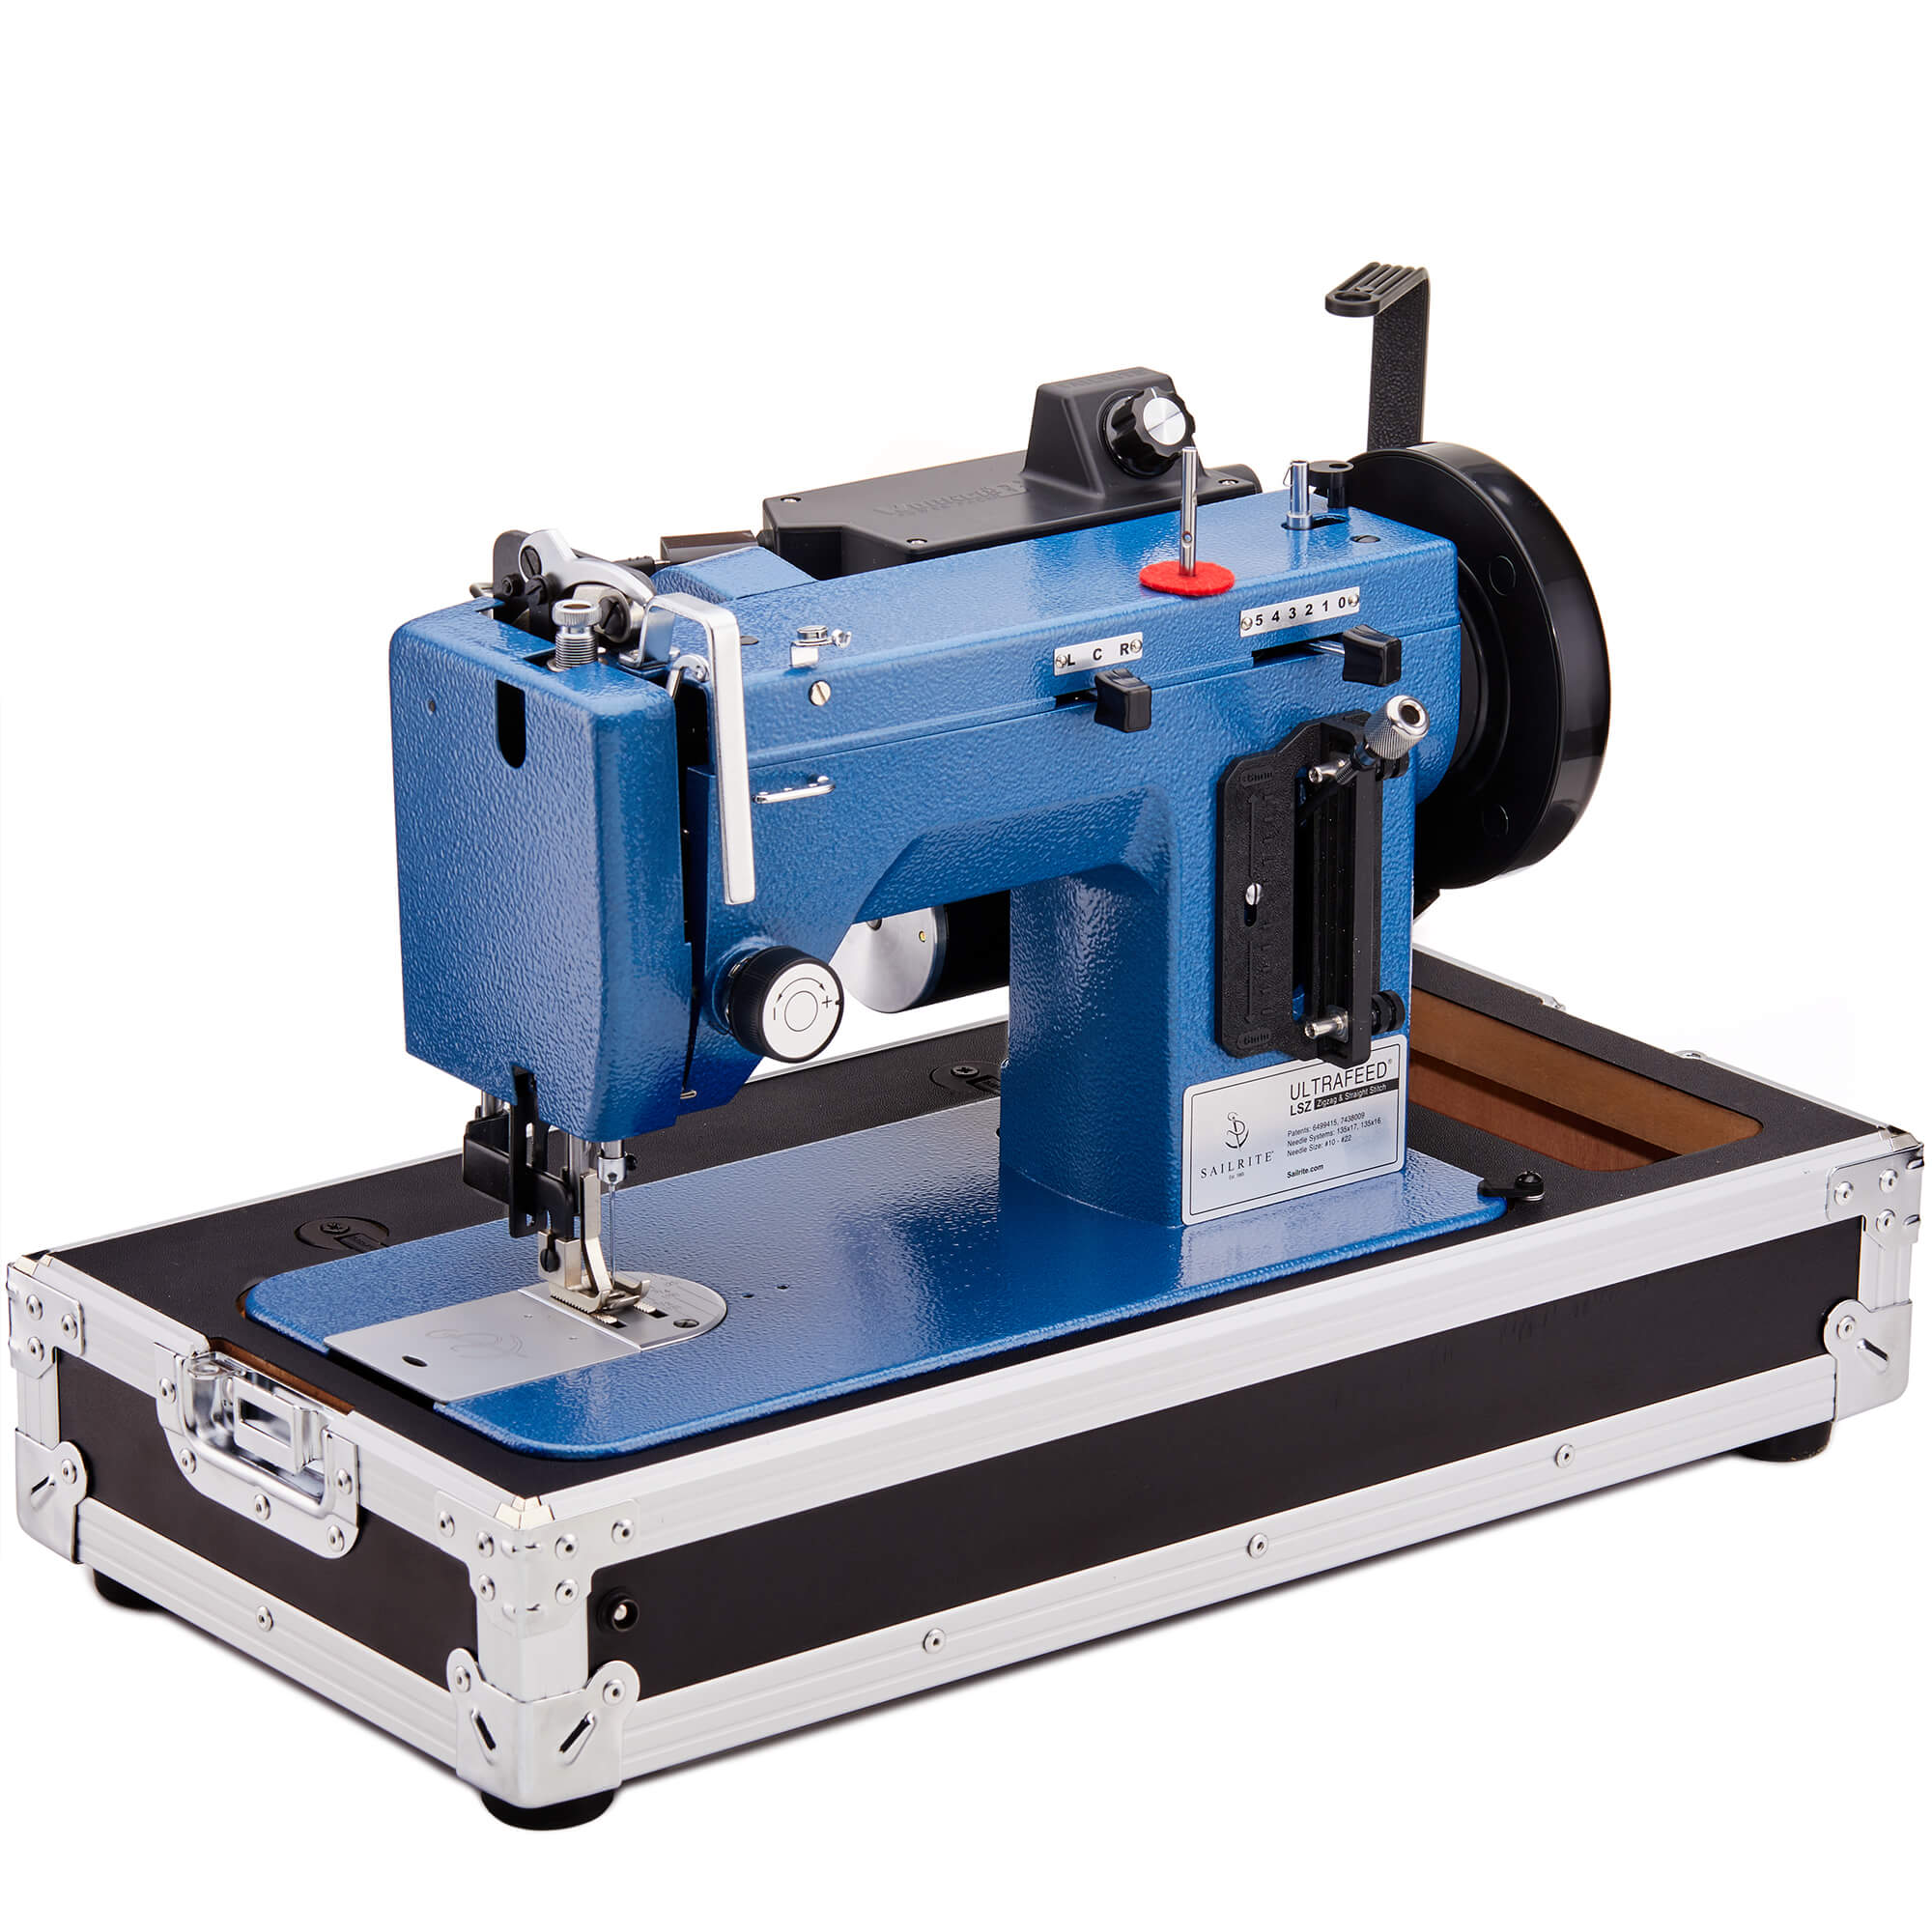
\includegraphics[width=0.6\textwidth]{images/sewing machine.jpg}
    \caption{Sewing machine}
    \label{fig:sew}
\end{figure}

\begin{figure}
    \centering
    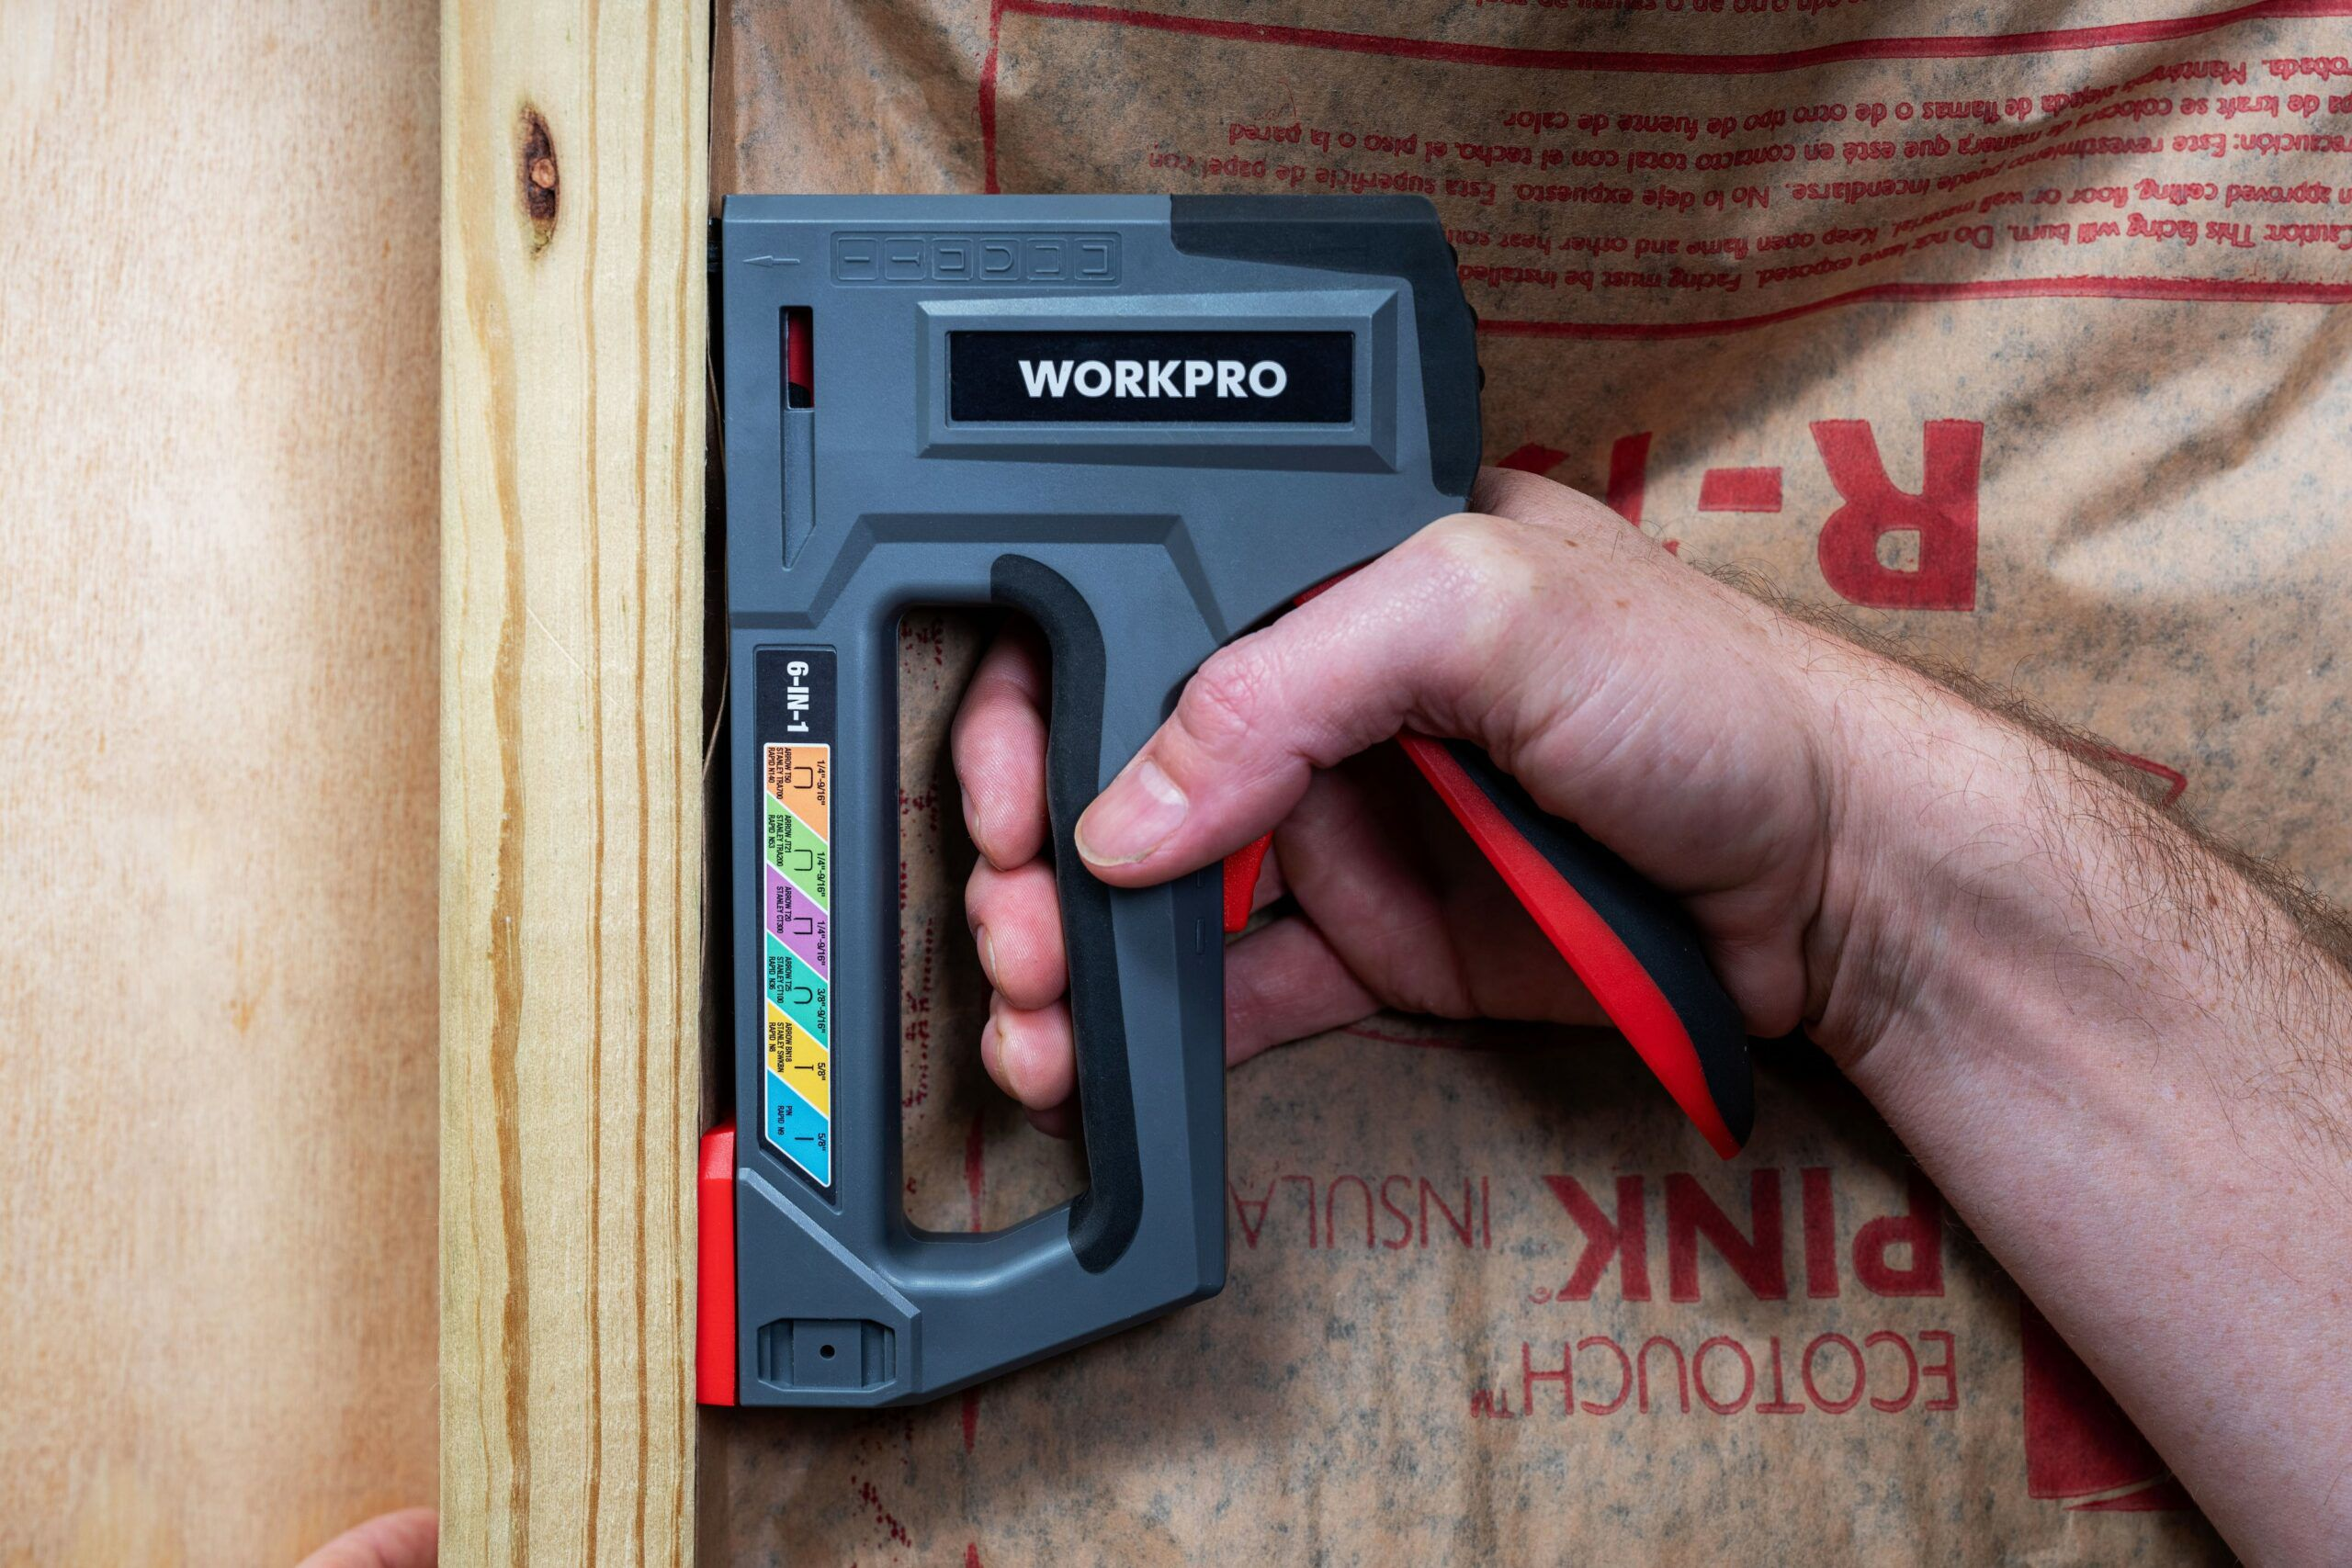
\includegraphics[width=0.6\textwidth]{images/staple gun.jpg}
    \caption{Staple gun}
    \label{fig:staple}
\end{figure}

\subsection{Installation and Assembly}
In this procedure, the parts produced in the previous steps will be assembled into the final product. The detail of the assembly line has been explained in Section \ref{sec:TechCon}. The machines and tools needed in this procedure include (shown in Figure \ref{fig:dns})
\begin{enumerate}
    \item Frame assembly station: Drill, rivet gun
    \item Recline mechanism installation station: Drill, screwdriver
    \item Cushion installation station: None (by hand)
    \item Armrest and desk assembly station: Screwdriver, drill
    \item Final assembly station: Screwdriver, drill
\end{enumerate}

\begin{figure}[!htp]
    \centering
    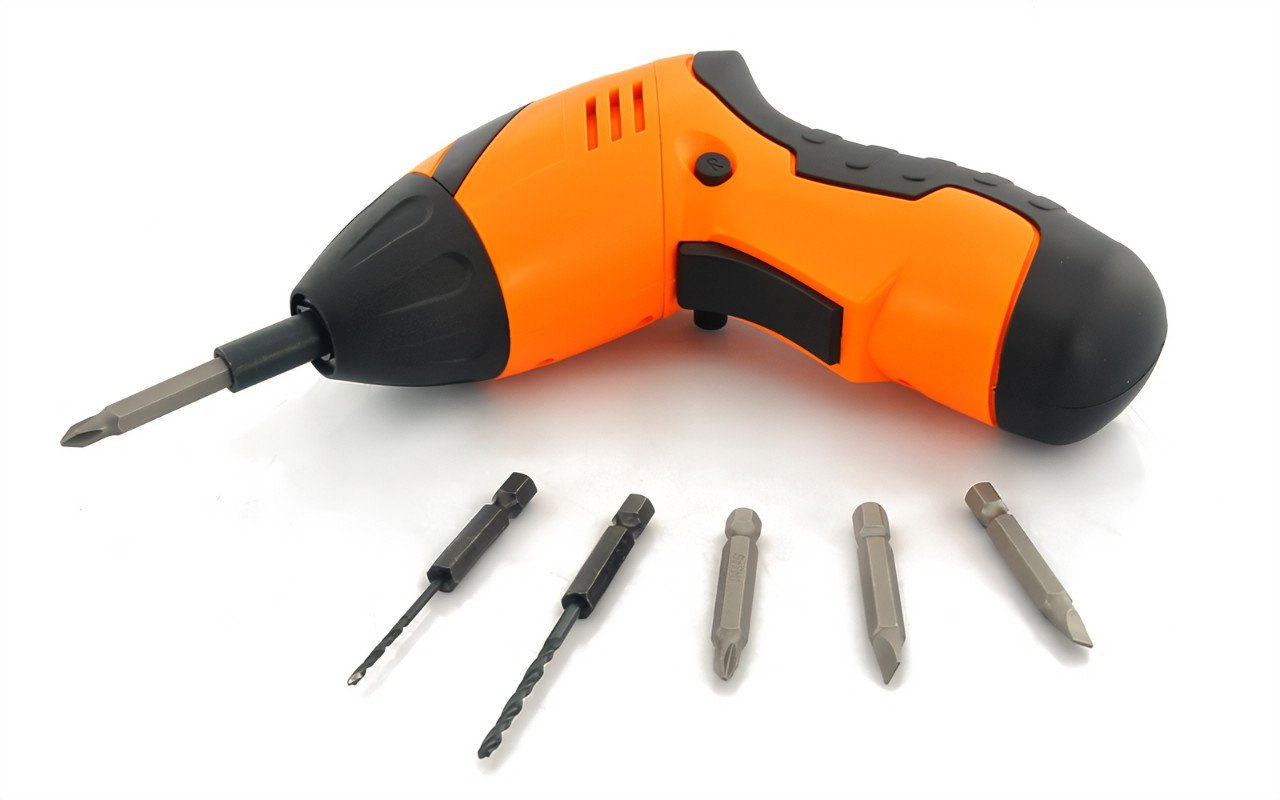
\includegraphics[width=0.6\textwidth]{images/dns.jpg}
    \caption{Drill and screwdriver}
    \label{fig:dns}
\end{figure}

\subsection{Quality Control} \label{sec:QC}
\begin{enumerate}
    \item \textbf{Dimensional check}: Verify that the width and height of the seat meet the specified dimensions.
    \item \textbf{Weight verification}: Ensure that the weight of the seat is within the specified range to ensure compatibility with the aircraft.
    \item \textbf{Frame inspection}: Test the strength of the frame by applying a load to the seat and checking for any signs of deformation or failure. Ensure all the parts of the frame, including the headrest frame, backrest frame, seat frame, armrests and desks won't detach under the load and torque.
    \item \textbf{Cushion quality check}: Check if the cushion covers are uniform and free from any blemishes, wrinkles, or tears. Test the 
    elasticity and softness of the polyurethane foam.
    \item \textbf{Recline function and armrests test}: Test the recline function and armrests to confirm that they operate smoothly and correctly. Confirm that they are adjustable within the designed range and not moveable without any limitations.
    \item \textbf{Modular component check}: Confirm that modular components, including cushions, covers, buttons, locking mechanisms, and other parts are assembled correctly and fit securely.
    \item \textbf{Foldable desk inspection}: Test the foldable desk to ensure that it functions as intended and is sturdy enough to support items within the designed load capacity.
    \item \textbf{Safety compliance check}: Confirm that the design meets all safety regulations and requirements, is crash-worthy, fire-resistant, and provides easy access to emergency exits in case of an emergency.
    \item \textbf{Cleaning and maintenance verification}: Ensure that the seat is designed for quick and easy maintenance, repair, and refurbishment and can be cleaned easily without causing damage to the seat.
\end{enumerate}